	\documentclass[10pt,a4paper]{report}
	\usepackage{graphicx}
	\usepackage[utf8]{inputenc}
	\usepackage{amssymb,amsmath}
	\usepackage{geometry}
	\usepackage[bookmarks=true]{hyperref}
	\usepackage{bookmark}
    \usepackage{wrapfig}
	%\geometry{article}
	\usepackage[ampersand]{easylist}	
    \newcommand\tab[1][1cm]{\hspace*{#1}}

\hypersetup{
	pdftitle={Digital integrated circuit design},%
	pdfauthor={Matteo Baldo},%
	pdfsubject={Digital integrated circuit design},%
	pdfkeywords={},%
	colorlinks=true,%
	linkcolor=blue,%
	linktocpage=true,%
	pageanchor=true
}


\begin{document}

% INIZIO PRIMA PAGINA DI INTRODUZIONE
\begin{titlepage}

	\centering
	{\scshape\huge\textbf Digital integrated circuit design \par}
	{\scshape\huge\textbf Notes \par}	
	\vspace{13cm}
{Professor:\\ \textit{Andrea Bonfanti}}	

\vspace{0.5cm}

{Student:\\ \textit{Matteo Baldo}}

\vspace{2cm}
	\vfill
	\raggedleft
	{\today\par}
	
\vspace{1cm}
\raggedright
{ \it ...and so on and so forth ...}
\end{titlepage}
% FINE PRIMA PAGINA DI INTRODUZIONE
        \newpage
		\setcounter{page}{2}
        \null 
        \thispagestyle{empty} 
        \newpage  


\pdfbookmark{\contentsname}{Index}
\tableofcontents
        % Intro page and index
%------------------------------------------------------------------------%
\chapter{Figures of merit in a digital integrated circuit}

        %Figures of merit in a digital integrated circuit
%------------------------------------------------------------------------%
\chapter{The MOS transistor}
\section{Symbols}
The symbols used to draw n and p MOS transistors in digital electronics are the one show in figure below

\centering
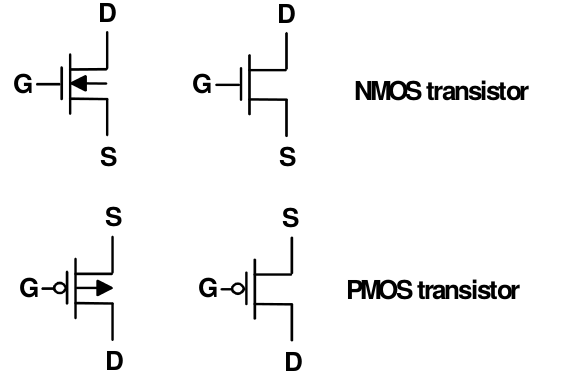
\includegraphics[width=0.35\textwidth]{C2_1.png}\\
\raggedright



\section{Working regimes}
We are intrested in the use of MOS transistors as swithces and not as amplifiers.\\
In our analysis we will consider the following operating regions with the corrisponding voltages 

\centering
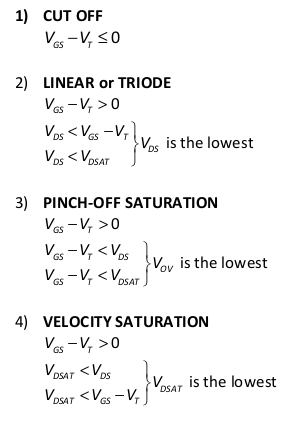
\includegraphics[width=0.3\textwidth]{C2_2.png}\\
\raggedright

and to assest the right expression of the current we will use the following unified model 


\centering
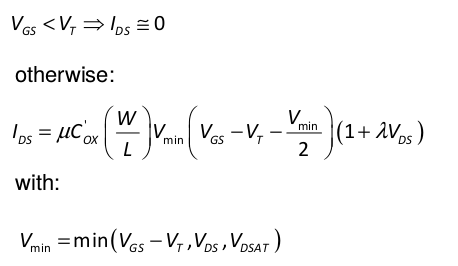
\includegraphics[width=0.5\textwidth]{C2_3.png}\\
\raggedright

In the reference technology of this course (bulk CMOS 0.25$\mu m$) this are the characteristics parameters

\centering
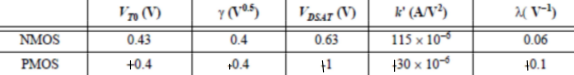
\includegraphics[width=0.7\textwidth]{C2_4.png}\\
\raggedright

\subsection{Body effect}

Since the $V_t$ depends on the source-body potential if this value is different form 0 we get

\centering
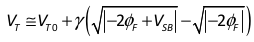
\includegraphics[width=0.35\textwidth]{C2_5.png}\\
\raggedright

where $\gamma$ is the body effect coefficient.

\subsection{Subthreshold regime}

When the overdrive voltage is equal to 0 the current in the device is not exactly 0 but the device enters in the so called subthreshold regime where the current behaves like in an BJT junction 

\centering
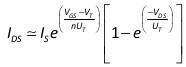
\includegraphics[width=0.35\textwidth]{C2_6.png}\\
\raggedright

this current is crucial in the power consumption in off mode.\\

\section{Equivalent resistance}
We can define an equivalent resistance of the MOS transistor as

\centering
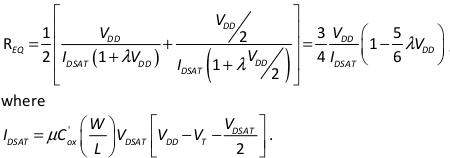
\includegraphics[width=0.5\textwidth]{C2_7.png}\\
\raggedright

the last term in parentesis can be easily neglected since is $\simeq 1$.\\
We can make three considerations:\\
\tab 1)the resistance is inversely proportional to the (W/L) ratio of the device\\
\tab 2)for $V_{DD} >> V_T + V_{DSAT}/2$, the resistance becomes virtually independent of the supply voltage\\
\tab 3)once the supply voltage approaches $V_{TE} =0.745V=V_T+V_{DSAT}/2$, a dramatic increase in resistance can be observed,even if the model adopted (considering the velocity saturation) is no longer valid\\
\vspace{5mm}
In digital electronics once we have the equivalent resistance of the MOS, we can evaluate the propagation time on the basis of the RC model, as $\ln(2)RC$.\\














        %The MOS transistor
%------------------------------------------------------------------------%
\chapter{The CMOS inverter}

\centering
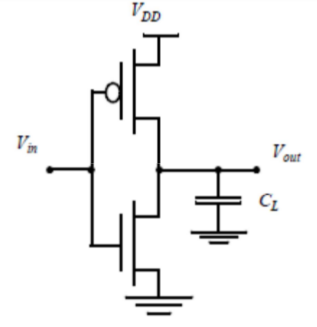
\includegraphics[width=0.35\textwidth]{C3_1.png}\\
\raggedright

We will refer to CMOS inverter implemented in a static FC-CMOS logic. FC-COMS means fully-complementary logic, which is a particular class of static gates.
Static refers to the fact that these gates have an output node always connected to GND or VDD through a low impedance path. Fully-complementary means that the gate is composed by a pull-down network and a complementary pull-up network.\\

\section{Static behavior}

Independently of the transistor size the high and low output levels are equal to $V_{DD}$ and GND that in out reference technology are 2.5V and 0V
\begin{equation}
V_{OH}=V_{DD}=2.5V
\end{equation}
\begin{equation}
V_{OL}=GND=0V
\end{equation}
This two values are indipentent form the relative device size; gates with this propriety are called ratioless (gates without this propriety are ratioead).\\
\vspace{5mm}
There is always in steady state a finite resistance between the output node and GDN or VDD (that isn't the equivalent resitance of the previous chapter that is useful to assest the propagation delay).\\
For VDD=2.5V we get
\begin{equation}
r_{on}=\frac{4.2k}{(W/L)_n}\ \ \ \ \ \ \ \ \ \ r_{on}=\frac{15.9k}{(W/L)_p} 
\end{equation}

\centering
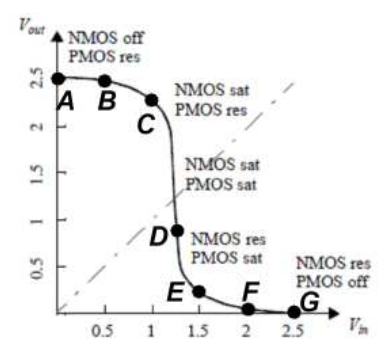
\includegraphics[width=0.35\textwidth]{C3_2.png}\\
\raggedright



\subsection{Switching threshold}
Let's suppose that during the transistion both transistor are in velocity saturation region (this is not correct but leads to a negligible error) to assest the threshold voltage $V_M$ of the inverter we have to put the 2 currents of the mos equal doing this we obtain 

\vspace{2.5mm}

\centering
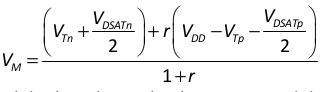
\includegraphics[width=0.35\textwidth]{C3_3.png}\\
\raggedright
 
with 

\centering
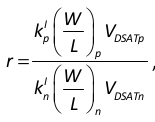
\includegraphics[width=0.15\textwidth]{C3_4.png}\\
\raggedright

We can oslo have the following inverse relationship

\vspace{2.5mm}

\centering
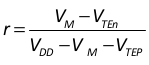
\includegraphics[width=0.15\textwidth]{C3_5.png}\\
\raggedright

For $V_M=1.25V$ that is the best case we get
\begin{equation}
\frac{(W/L)_p}{(W/L)_n}=3.5\simeq 3
\end{equation}

\subsection{Noise marigns}

To compute $V_{IL}$, $V_{IH}$ we consider the piecewise linear approximation for the VTC, where the transition region is approximated by a straight line having the same negative slope of original VTC in the threshold point.\\

\centering
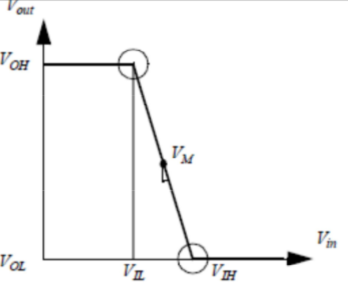
\includegraphics[width=0.35\textwidth]{C3_6.png}\\
\raggedright

In this way the straight line that approximates the VTC near the threshold is 
\begin{equation}
V_{OUT}=V_{IN}g+(1-g)V_M \ \ \ \ \ \ (g<0)
\end{equation}
we can compute g considering that $g=-(g_{mn}+g_{mp})r_{0p}//r_{0p}$ we obtain

\vspace{2.5mm}

\centering
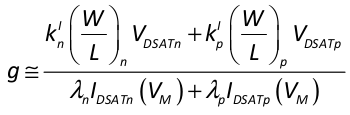
\includegraphics[width=0.35\textwidth]{C3_7.png}\\
\raggedright

\vspace{2.5mm}

The gain is apporoximately constant if the velocity saturation is taken into account.\\

From this we get 

\centering
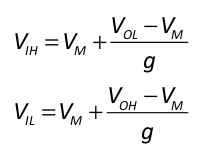
\includegraphics[width=0.15\textwidth]{C3_8.png}\\
\raggedright

\centering
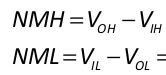
\includegraphics[width=0.11\textwidth]{C3_9.png}\\
\raggedright

\section{Dinamic behavior}


\centering
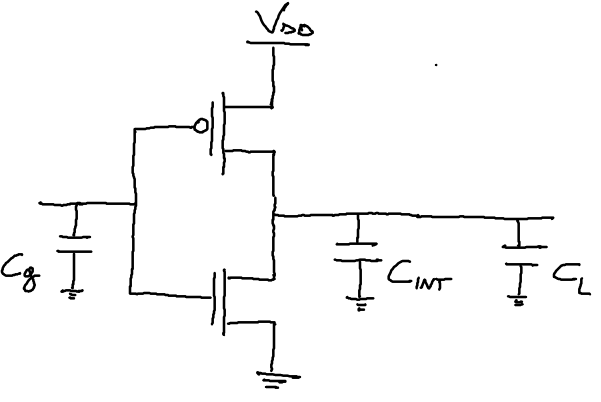
\includegraphics[width=0.45\textwidth]{C3_10.png}\\
\raggedright

We define the following parameters \\
\tab $W_n,W_p$ the width of the drain junctions (that is the same of W/L)\\
\tab $L_D$ Drain length (that isn't the same as W/L)\\
\tab $A_{d}=W*L_D$ the area of the drain\\
\tab $P_{d}=2L_D+W$ the perimeter of the drain\\


\subsection{Intinsic capacitance $C_{int}$}
\vspace{2mm}
\begin{equation}
C_{int}=C_{overlap}+C_{dbn}+C_{dbSWn}+C_{dbp}C_{dbSWp}
\end{equation}
{\bf Overlap capacitance}\\
\begin{equation}
C_{ovelap}=2(C'_{ovp}W_p+C'_{ovn}W_n)
\end{equation}
\vspace{5mm}
{\bf Drain-bulk n capacitances}
\begin{equation}
C_{dbn}=\frac{C'_{jn}A_{dn}}{2}\left(\frac{1}{(1+\frac{V_{DD}}{\phi})^{0.5}}+\frac{1}{(1+\frac{V_{DD}}{2\phi})^{0.5}}  \right)
\end{equation}

\begin{equation}
C_{dbSWn}=\frac{C'_{jSWn}P_{dn}}{2}\left(\frac{1}{(1+\frac{V_{DD}}{\phi})^{0.44}}+\frac{1}{(1+\frac{V_{DD}}{2\phi})^{0.44}}  \right)
\end{equation}

\vspace{5mm}
{\bf Drain-bulk p capacitances}
\begin{equation}
C_{dbp}=\frac{C'_{jp}A_{dp}}{2}\left(1+\frac{1}{(1+\frac{V_{DD}}{2\phi})^{0.48}}  \right)
\end{equation}

\begin{equation}
C_{dbp}=\frac{C'_{jSWp}P_{dp}}{2}\left(1+\frac{1}{(1+\frac{V_{DD}}{2\phi})^{0.32}}  \right)
\end{equation}


\subsection{Gate capacitance $C_{g}$}

\begin{equation}
C_g=C'_{ovn}W_n+C'_{ovp}W_p+C'_{ox}(W_nL_n+W_pL_p)
\end{equation}

\subsection{Self-loading factor}
We can define the self-loading factor $\gamma$ as 
\begin{equation}
C_{int}=\gamma C_g
\end{equation}
In our reference technology we have $\gamma=1$ and $C_g^{(1)}=2fF$ where the suffix (1) is the size of the inverter (that is the W/L of the n-mos).\\
If we have an inverter of size $\alpha$ it's gate capacitance will be 
\begin{equation}
C_g^{(\alpha)}=\alpha C_g^{(1)}=\alpha\cdot 2fF
\end{equation}


\section{Propagation delay}
\centering
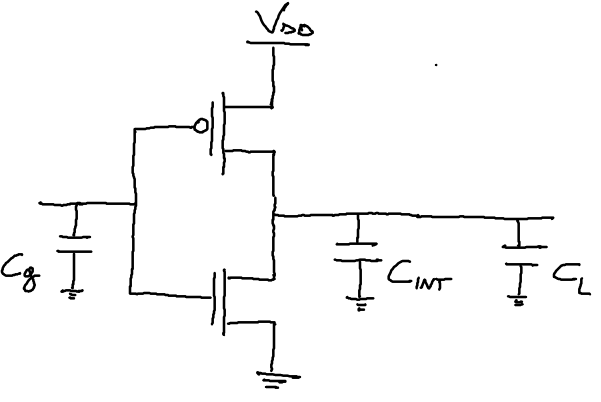
\includegraphics[width=0.45\textwidth]{C3_10.png}\\
\raggedright

Propagation delay form high to low

\centering
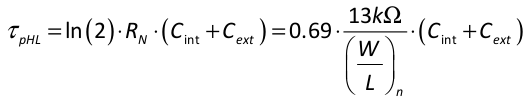
\includegraphics[width=0.35\textwidth]{C3_11.png}\\
\raggedright

\vspace{5mm}

Propagation delay forom low to high 

\centering
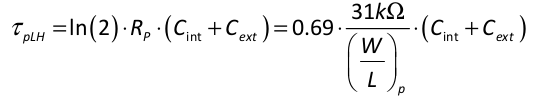
\includegraphics[width=0.35\textwidth]{C3_12.png}\\
\raggedright

\vspace{5mm}
We define intrinsic propagation delay as the average between this 2 results when $C_{ext}=0$
\begin{equation}
\tau_{p0}=\frac{\tau_{HL}+\tau_{LH}}{2}
\end{equation}

\subsection{Fan-out}
Considering an external capacitance we get the folowing expression
\begin{equation}
\tau_p=\ln(2)R_{eq}(C_{int}+C_{ext})=\tau_{p0}\left(1+\frac{C_{ext}}{C_{int}}\right)=\tau_{p0}\left(1+\frac{C_{ext}}{\gamma C_g}\right)=\tau_{p0}\left(1+\frac{f}{\gamma}\right)
\end{equation}
Where we used the fan-out f and the self-loading factor defined as
\begin{equation}
f=\frac{C_{ext}}{C_g}\ \ \ \ \ \ \ \ \ \ \ \ C_{int}=\gamma C_g
\end{equation}

\section{Chain of inverters}

To optimize the propagation delay of an inverter chain with N elements we have to set all propagation delay of the inverters equal $f_i=f_i+1\ \ \  \forall i=0,...,N$.\\
To do this we have to calculate the path fan-out that is the load over the first gate capcitance
\begin{equation}
F=\frac{C_L}{C_{g,1}}
\end{equation} 
And from this we calculate the optimum fan-out 
\begin{equation}
f_{opt}=\sqrt[N]{F}
\end{equation}
given the first inverter size $s_1$ all the other inverters' dimensions are fixed 
\begin{equation}
s_n=s_1\cdot (f_{opt})^{n} \ \ \ \forall n=1,...,N 
\end{equation} 
and the propagation delay is 
\begin{equation}
\tau_p=N\tau_{p0}\left(1+\frac{f_{opt}}{\gamma} \right)
\end{equation}

\vspace{5mm}

If the number of inverter isn't fixed we can compute for our reference technology the optimum number of stages as 
\begin{equation}
N_{opt}=\frac{\ln(F)}{\ln(3.6)}
\end{equation}
beacuse the best fan-out that we can have is 
\begin{equation}
f_{opt}^{ideal}=3.6
\end{equation}
Of course the number of stages N has to ben an integer number.\\

        %The CMOS inverter
%------------------------------------------------------------------------%
\chapter{Inverter power consumption}

\section{Dynamic power consumtion}
Only in case of charge of a capacitance so in a LOW to HIGH transition at the output of an inverter. \\
The most general formula for the power dissipated in this process is
\begin{equation}
P_{dyn}=C_LV_{DD}^2f_{1\rightarrow 0}
\end{equation}
where $f_{1\rightarrow 0}$ is the frequency of the 0-1 transition at the output node. This term can be deconposed in 2 factor the clock of the circuit and the switching activity $\alpha_{SW}$ that is the probability to have a transition from 0 to 1 at the output.\\
\vspace{2mm}
\tab In case of a square wave we have 
\begin{equation}
f_{1\rightarrow 0}=f_{clk}\cdot \alpha_{SW}=f_{clk}\cdot \frac{1}{2}
\end{equation}
\tab In case of a randoom signal 
\begin{equation}
f_{1\rightarrow 0}=f_{clk}\cdot \alpha_{SW}=f_{clk}\cdot \frac{1}{4}
\end{equation}
\vspace{5mm}
In the end we can write this 2 final equation for dynamic power dissipation
\begin{equation}
P_{dyn}=C_LV_{DD}^2 f_{clk}\cdot \alpha_{SW}
\end{equation}
\begin{equation}
E_{dyn}=C_LV_{DD}^2\alpha_{SW}
\end{equation}
In case of a chain of inverters $C_L$ is the sum of all the capacitance at the output nodes of the single inverters.\\

\section{Cross-conduction power consumption}
Due to the finite slope of the input signal there is a finite time when both p-mos and -mos are on creating a low impedance path between $V_{DD}$ and GND.\\

\centering
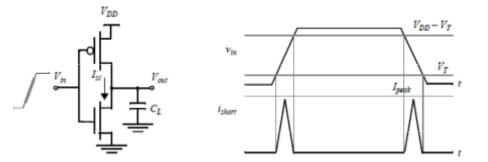
\includegraphics[width=0.7\textwidth]{C4_1.png}\\
\raggedright

\centering
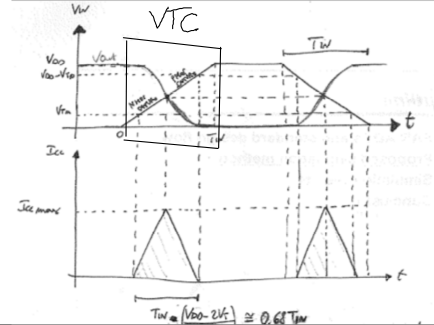
\includegraphics[width=0.5\textwidth]{C4_1b.png}\\
\raggedright

Defining $T_{in}$ as the time needed by the input signal to transition from GND to $V_{DD}$ and vice-versa and $I_{peak}$ the velocity saturation current of the n-mos (when the input and the output are at $V_m$) we can compute the cross-conduction energy as (assuming $V_{tp}=V_{tn}$) 
\begin{equation}
E_{cc}= \frac{1}{2} V_{DD}I_{peak}\cdot 0.68 \cdot T_{in}
\end{equation}
If we consider an input signal with an update frequency of f with continuos switch HL LH the power is 
\begin{equation}
P_{cc}=\frac{V_{DD}I_{peak} \cdot 0.68 \cdot T_{in}}{2} f
\end{equation}

\vspace{5mm}

With capacitve loads the cross-conduction power becomes smaller than without.\\ 
The cross conduction power can be neglected when 
\begin{equation}
T_{in}<10\tau_p
\end{equation}
with $\tau_p$ propagation delay of the stage.\\


\section{Static power consumption}
It's due to the subthreshold current of the MOS devices.

        %Inverter power consumption
%------------------------------------------------------------------------%
\chapter{The wires}

To simplify the analysis of the wires parasitics effects we introduce 3 simple assumption;\\
\vspace{2mm}
\tab $\rightarrow$ Inductance can be neglected if the wire resistance is large or if the rise/fall time of the input signal is large.\\
\vspace{2mm}
\tab $\rightarrow$ When the wire is short and when the equivalent resistance of the driver is large, the wire resistance can be serenely neglected.\\
\vspace{2mm}
\tab $\rightarrow$ When the separation between nearby wires is large or when the wires run in parallel for a short distance, the inter-wires capacitance can be neglected.\\


%------------------------------------------------------------------------%
%------------------------------------------------------------------------%
\section{Capacitance}

\centering
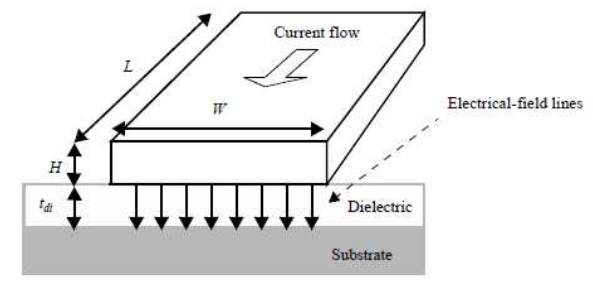
\includegraphics[width=0.5\textwidth]{C5_1.png}\\
\raggedright

We divide the overall capacitance of a wire in 2 main contribution; parallel plate capacitance and fringing capacitance.\\
In the ideal case where the parameter $W/t_{di}$ is very large the fringing capacitance contribution can be neglected but since in our reference technology we can have $W/H>1$ the fringing or border capacitance is the dominant contribution.\\
\vspace{5mm}

For our reference technology process the following table is given reporting the parallel-plate and the fringing capacitance contributions for a wire in a certain layer with respect to another wire in another layer.\\
The parallel-plate capacitance is reported in the white rows expressed in $aF/\mu m^2$ of overlapping area, while the shaded rows report the fringing capacitance contribution in $aF/\mu m$ of perimeter (that is quite always $\simeq 2L$).\\

\centering
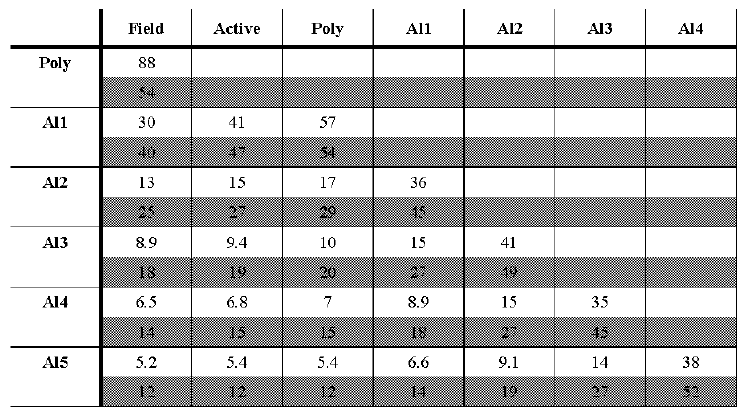
\includegraphics[width=0.8  \textwidth]{C5_2.png}\\
\raggedright
When using this table we have always to look what tipe of metal is our wire (rows) and in what material is made the ground plane or the other wire (columns) in order to get the correct values.\\

\vspace{3mm}
To evaluate che capacitance of 2 nearby wires implemented in the same layer at minimum distance we get the following table with the vales of the capacitances for unit lenght expressed in $aF/\mu m$ \\
\vspace{3mm}

\centering
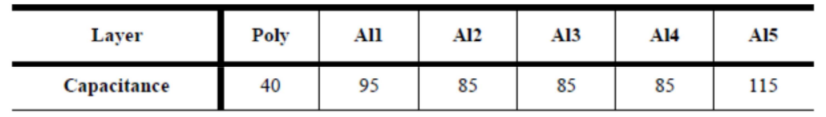
\includegraphics[width=0.8\textwidth]{C5_3.png}\\
\raggedright


%------------------------------------------------------------------------%
%------------------------------------------------------------------------%
\section{Resistance}

Resistance of a wire can be assested as
\begin{equation}
R=\rho \frac{L}{WH}=R_{sh}\frac{L}{W}
\end{equation} 
where the last part represent the resistance per square multiplied by the number of squares.\\
\vspace{5mm}
At very high frequency, the resistance tends to increase due to the skin effect. In practice the current tends to flow in the peripheral part of the wire. Considering a wire with a width W and a height H, the current flows almost entirely in a peripheral section characterized by a depth
\begin{equation}
\sigma=\sqrt{\frac{\rho}{\pi f \mu }}
\end{equation}
if the wire is smaller than the skin effect at a given frequency there are no difference in the resistance. It's an effect that affects only wide wires.\\


%------------------------------------------------------------------------%
%------------------------------------------------------------------------%
\section{Models for wires}



\subsection{Lumped C model}
Since the resistance of the wire is much smaller wrt the driving resitance we can model the wire with only it's capacitance.

\centering
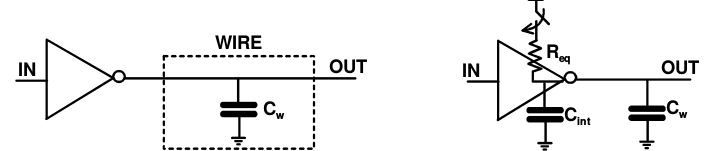
\includegraphics[width=0.5\textwidth]{C5_4.png}\\
\raggedright

The wire capacitance has to be added to the intrinsic capacitance of the inverter in order to correctly estimate the propagation delay that in this case is 
\begin{equation}
\tau=\ln(2)R_{eq}(C_{int}+C_w)
\end{equation}



\subsection{Lumped RC model}
When the resistance is no more negligible a first odrer approximation is to model the wire as it's single equivalent resistace and capacitance 

\centering
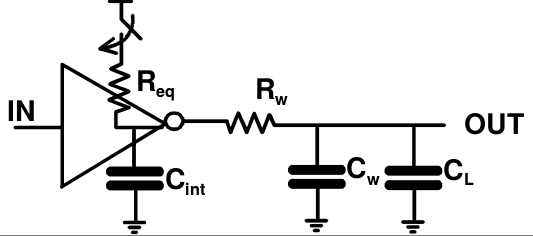
\includegraphics[width=0.35\textwidth]{C5_5.png}\\
\raggedright

To estimate the overall propagation we can model the circuit as follows and use the Elmore theorem

\centering
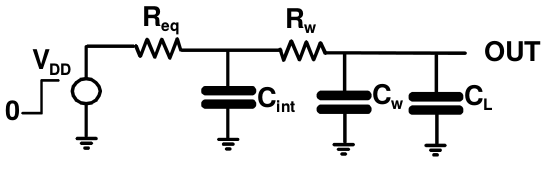
\includegraphics[width=0.35\textwidth]{C5_6.png}\\
\raggedright


\centering

\fbox{\begin{minipage}{40em}
\centering
{\bf Elmore theorem}\\
\raggedright
With a network that has a single input node ,all capacitance between a node and ground and no resistive loops we can assest the propagation delay of the line as calculating for every capacitance C of the network the so called shared-path resistance. This resistance represents the resistance shared between the path from the source of the signal and the output and the path form the source to the capacitance.\\

\centering
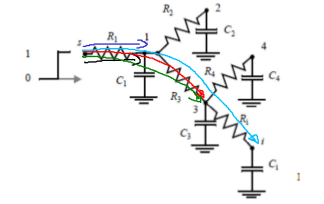
\includegraphics[width=0.35\textwidth]{C5_7.png}\\
\raggedright

\begin{equation}
\tau=C_1R_1+C_2R_1+C_3(R_1+R_3)+C_4(R_1+R_3)+C_j(R_1+R_2+R_j)
\end{equation}

\end{minipage}}

\raggedright
\vspace{5mm}

This is an approximation that brings us to an overestimation of the propagation delay (factor 2) beacuse we are supposing all parasitic terms concentrated in one point and not distributed over a line.\\

\subsection{Distributed model}
With the distributed model we divide the wire into lot of wires of length $\Delta L$ with $\Delta L \rightarrow 0$.\\

\centering
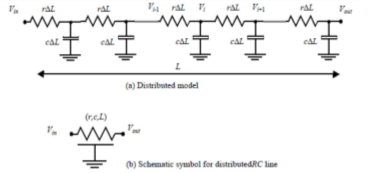
\includegraphics[width=0.5\textwidth]{C5_8.png}\\
\raggedright

In this way through the resoluton of a differential equation for the voltage over the line we get that the delay of the wire is 
\begin{equation}
\tau_w\simeq \ln(2)\frac{R_wC_w}{2}
\end{equation}
That is the correct value wrt the lumped RC model.\\

To correctly take into account the effects of the distribution we will use the following 2 models that give us both the same result of the distributed model

\centering
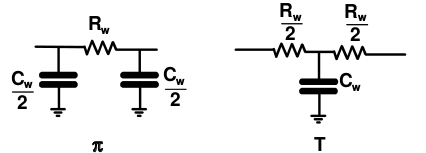
\includegraphics[width=0.35\textwidth]{C5_9.png}\\
\raggedright


\section{Buffering of a line}

If the time constant of a line it's the dominant contribution for delay in our digital circuit it's worth in order to get a faster respnce to cut the wire in N pieces adding buffer in the middle.\\
This is convenient if
\begin{equation}
L\ge\sqrt{\frac{16C_{int}R_{eq}}{cr}}
\end{equation}
where $C_{int},R_{eq}$ are parameters of the driving circuit and c,r are the specific resistance ($\Omega/m$) and capacitance ($F/m$) of the wire.
The optimum number of division N (and so the number of inverter to be added N-1) is
\begin{equation}
N=\sqrt{\frac{R_wC_w}{4C_{int}R_{eq}}}=L\sqrt{\frac{rc}{4C_{int}R_{eq}}}
\end{equation}
And the contribution to $\tau_p$ of the wire ($R_wC_w/2$) decreases by a factor N.\\
The propagation delay of an optimized line that is broken in N peices is 
\begin{equation}
\tau_p=\ln(2) N \left(R_{eq}C_{int}+(R_{eq}+\frac{R_w}{2N})\frac{C_w}{N}+(R_{eq}+\frac{R_w}{N})C_{int}\right)
\end{equation}
In this expression we supposed inverters with the same size and $\gamma=1$.\\
This optimization of the line it's indipendent form the size of the stage present in the circuit.\\

\section{Inductance}

Parasitic inductances can be neglected if the time of flight of the signal is much less than the minimum propagation delay of the circuit. With a line of length L and the maximum propagation delay of $\tau_{max}$ this translates as 
\begin{equation}
t_{flight}=\frac{L}{\frac{c}{\sqrt{\mu \varepsilon}}}\ \  << \ \ \tau_{max}     
\end{equation}
where tipically $\varepsilon=3.9$.\\
\vspace{5mm}
Another condition that makes the inductance negligible is to have
\begin{equation}
L\ \ <<\ \ \frac{1}{r}\sqrt{\frac{l}{c}}
\end{equation}
where r, l and c are the specific resistance inductance and capacitance.\\
        %The wires
%------------------------------------------------------------------------%
\chapter{FC-CMOS gates}

\section{Sizing of single transistor inside a logic gate}
Once the transistor are placed in order to compute the requested logic function the sizing of the single transistor has to follow this simple rule: the equivalent resistance in the worst case state has to be equal to the one of an inverter of the same size of the gate.\\
Transistor in parallel show a resistance half of a single transistor so considering the following NAND gate with a size equal to 1 the p-mos will have an aspect ratio of 3 and the n-mos of 2 (two transistor of size 2 in series are the equivalent of a transistor of size 1).\\

\centering
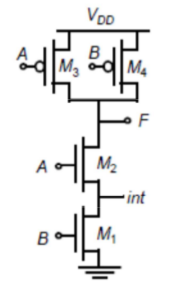
\includegraphics[width=0.15\textwidth]{C6_1.png}\\
\raggedright

If the searched size was s=2 we will have p-mos 6 and n-mos 4 of aspect ratio.\\

\section{Equivalent capacitance}
To estimate the equivalent internal capacitance $C_{int}$ of a generic FC-CMOS gate we have to look to the dimesnions of the transistors connected to the output node. The sum of the aspect ratios of this transistors divided by 4 it's how many $C_g^{(0)}$ the internal capacitance is.\\
\vspace{5mm}
To better assest the propagation delay we should also take into account the inter-nodes capacitance inside our gate; this leads us to a more complex analysis since we have to consider whitch parasitic capacitance are charged an whitch are discharged and we shoulde use the Elmore theorem for every transistion.

\centering
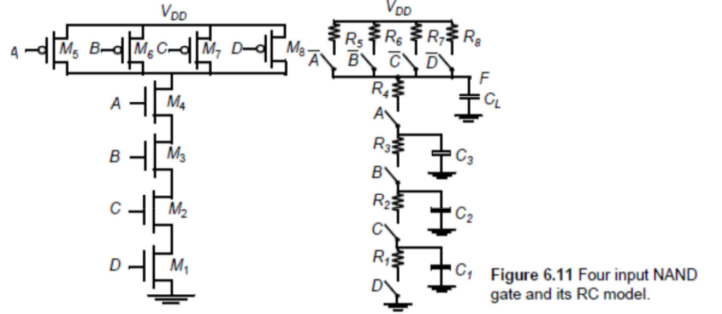
\includegraphics[width=0.5\textwidth]{C6_2.png}\\
\raggedright

This inter-nodes capacitance can't be estimated as before with a value of 2fF but , since 2 transistor in series are integrated with common drain-source, with 1fF capacitance.\\


\centering
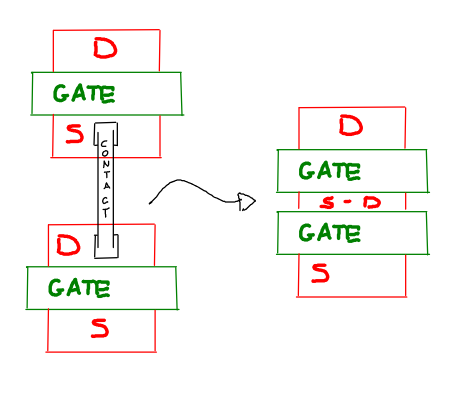
\includegraphics[width=0.35\textwidth]{C6_3.png}\\
\raggedright

We can neglect the effect of the inter-nodes capacitance since our gates have small fan-in (3-4 max).\\

\vspace{5mm}
In case of large fan-in and a lot of transistors in series it's possible to adopt clever sizing "inspired" by the inverter chain optimization 

\centering
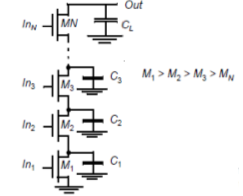
\includegraphics[width=0.35\textwidth]{C6_4.png}\\
\raggedright

\vspace{5mm}
Another good rule of thumb is that the last signal coming to the gate (the slowest signal at the input of the gate) has to be connected to the transistor closest to the output.\\

\section{Propagation delay}

\subsection{Equivalent resistance}
We define the equivalent resistance of a generic gate of size s (built with the right internal proportion described before) as 
\begin{equation}
R_{eq}=\frac{R_{eq}^{(1)}}{s}=\frac{11.6k\Omega}{s}
\end{equation}

\subsection{"p" factor}
The factor "p" or intrinsic delay factor (OUTPUT) it's a constant that connect the intrinsic capacitance of our gate with the intrinsic capacitance of an inverter of the same dimensions and can be calculated as 
\begin{equation}
p=\frac{C_{int}(s=1)}{C_{int}^{(1)}}
\end{equation}
\begin{equation}
p=\frac{\sum \frac{W}{L}|_{mos \ connected \ to \ y}}{4*s}
\end{equation}
and it's releted with the intrinsic capacitance of a generic size gate as 
\begin{equation}
C_{int}=spC_{int}^{(1)}
\end{equation}
This parameter it's indipendent on the size of the gate

\subsection{"g" factor}
The factor "g" is the logical effort (INPUT) that quantifies the complexity of the gate with respect to the inverter in the "input" direction.\\
Also this parameter is indipendent on size and has to be calculated considering single couple of inputs\\ 
\begin{equation}
g=p=\frac{C_{g}(s=1)}{C_{g}^{(1)}}
\end{equation}
\begin{equation}
g=\frac{\sum \frac{W}{L}|_{mos \ connected \ to \ A}}{4*s}
\end{equation}


\vspace{6mm}
\centering
Here some examples of this parameters on famous logic gates\\
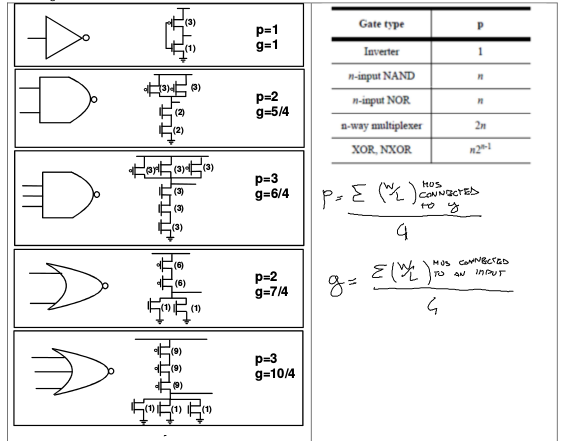
\includegraphics[width=0.75\textwidth]{C6_5.png}\\
\raggedright

\subsection{Propagation delay}
The expression of the propagation delay of a generic gate is
\begin{equation}
\tau_p=\tau_{p0}\left(p+\frac{fg}{\gamma}\right)
\end{equation}
where we can distinguish two contributions; the term $\tau_{p0}$ is the intrinsic delay and $fg\tau_{p0}$  is the effort delay strictly related to the load capacitance. The product fg it's called stage effort or h.\\

\section{Size optimization of $\tau_p$}
The delay that counts and that we are going to optimize it the one related with the critical path, the delay of the longest path.\\
To optimize the propagation delay we need that all the gates have the same stage effort h.\\
\vspace{5mm}
We define the path fan-out as 
\begin{equation}
F=\frac{C_L}{C_{g,1}}
\end{equation}
and the path logical effort as 
\begin{equation}
G=\prod g_i
\end{equation}
To optimize the propagation delay we all the stages has to have the following $h_{opt}$
\begin{equation}
h_{opt}=\sqrt[N]{H}
\end{equation}
This corresponds to a propagation delay of the overall chain of 
\begin{equation}
\tau_{p,opt}=\tau_{p0}\left( (\sum p)+\frac{N h_{opt}}{\gamma} \right)
\end{equation}
in this way the dimension of the j-th stage will be 
\begin{equation}
s_j=\frac{s_1g_1}{g_j}\prod_{i=1}^{j-1}f_i
\end{equation}
or better we can assest every dimension form the first stage to the last one using the formula of $h_{opt}$
\begin{equation}
h_{opt}=f_ig_i \ \ \ \forall i
\end{equation}
using this formula on the i-th stage we will end up with the size of the i+1 stage.

\subsection{Branching}
In the case illustrated in figure we have a so called branching in the path.

\centering
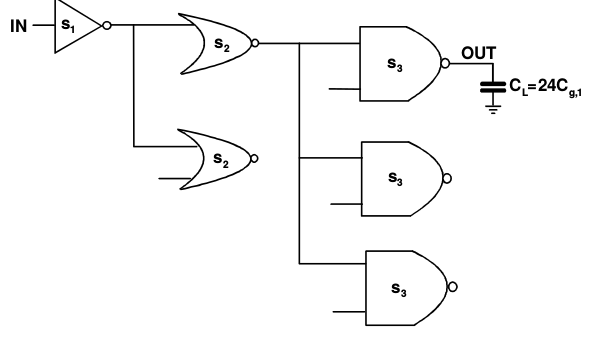
\includegraphics[width=0.35\textwidth]{C6_6.png}\\
\raggedright

There are more stages in parallel (NAND in this case). Under the assumption that all the parallel elements have the same dimensions (all NAND with equal size) we can define the branching factor refering to the extrinsic capacitance as b
\begin{equation}
b=\frac{C_{path}+C_{off-path}}{C_{path}}
\end{equation}
that in practice is the number of stages in parallel (3 in our case).\\
\vspace{5mm}
In this cases we can optimize the chain introducing the path branching factor B
\begin{equation}
B=\prod_{i=1}^N b
\end{equation}
than the way to optimize the chain is the same as before but the H is now defined as 
\begin{equation}
H=FGB
\end{equation}
the number of stages n does not takes into account the braching stages and so to find the size of the single stages we can use the relation
\begin{equation}
h_{opt}=\sqrt[n]{H}=f_ig_ib_i
\end{equation}


\section{Power dissipation}
The consideration on power dissipation are the same for the simple NOT circuits we've done in the previous chapter. The difficult topic here is to assest the parameter $\alpha_{sw}$ and to reason if some states are correleted each other.
\vspace{5mm}
Assuming that the inputs are independent and uniformly distributed, any N-input static gate has a transition probability that corresponds to
\begin{equation}
\alpha_{sw}=\frac{N_0N_1}{2^{2N}}=\frac{N_0(2^N-N_0)}{2^{2N}}
\end{equation}
where $N_0$ and $N_1$ are the number of zero and one, respectively, in the truth table of the logic function.
\vspace{5mm}
Here follows an example where the above formula doesn't work since the 2 inputs are correlated


\centering
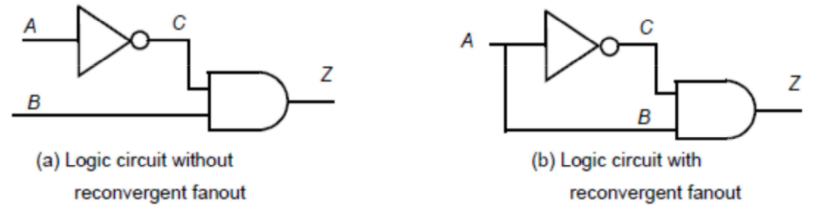
\includegraphics[width=0.7\textwidth]{C6_7.png}\\
\raggedright




















        %FC-CMOS gates
%------------------------------------------------------------------------%




\end{document}
